\subsection{Ethylene pyrolysis in a flow reactor}
The PFR model was used to simulate the pyrolysis of \%0.6 $\mathrm{C_2H_4-N_2}$ in a flow reactor 1.4 m long and 16 mm in diameter. Figure~\ref{fig:pfr_temp} shows the axial temperature profile with the maximum temperature, $\mathrm{T_{max}}$ of 1673 K imposed on the model, which was calculated based on the thermocouple measurements by~\citet{mei2019quantitative} for various flow rates along the reactor centerline. The temperature starts from 300 K at the entrance and increases to reach the hot zone with the temperature within 10\% of $\mathrm{T_{max}}$.  The length of hot zone changes from 0.71 m for Q=8 L/min to 0.76 m for Q=12 L/min due to the advection effect. The temperature drop to 650 K near the end of the reactor. 

The inception and PAH adsorption adjustment factors were varied to match the predicted PSD with measurements at the end of reactor for various volumetric flow rates, Q of 8.5, 11 and 12 L/min shown in Figure~\ref{fig:pfr_psd}. The parametric analysis showed that only a single set of adjustment factors exist for each inception model that minimizes the prediction error of PSD across the flow rates. The KAUST mechanism~\citep{wang2013pah} was used to describe gas chemistry as it results in better agreement with PSD measurements compared to Caltech. A bimodal size distribution can be observed for Q=8 L/min (Figure~\ref{fig:pfr_psd}-a) that was attributed to the continuous inception~\citep{zhao2003measurement}. The comparison of simulations with measurements reveals different temperature dependence of inception models. Irreversible Dimerization and Dimer Coalescence (irreversible inception models) capture the bimodality of PSD in good agreement with the measurements, but the other two models predict a nearly unimodal PSD. The number concentration of the first section is lower by more than three orders of magnitude for Reactive Dimerization and EBridge Modified indicating the lack of active inception at the sampling location due the temperature drop near the end of reactor that suppresses soot inception.

All inception models captured the disappearance of shoulder in the PSD at 11 and 12 L/min because the particle residence time is shorter compared to 8 L/min and the sampling was done before coagulation becomes dominant and forms the second peak. However, a one order of magnitude underprediction of the number concentration of incipient particles by Reactive Dimerization and EBridge Modified are compared to two irreversible inception models.

Figure~\ref{fig:pfr_psd} shows the evolution of total number concentration of agglomerates, $N_{agg}$ along the reactor. The predictions of the inception models are relatively close until z$\approx$1.1 m that corresponds to end of hot zone in the reactor, but $N_{agg}$ grows for irreversible inception models beyond that point because the inception continues in the low temperature region. The irreversible models are in better agreement with  measurements for 8 and 11 L/min, but overestimate the final number concentration at 12 L/min.

As shown in Figure\ref{fig:pfr_Iinc}, soot inception flux exhibits a sharp increase as the flow enters the hot zone of the reactor. The axial distance at which inception flux exceeds $10^7$ is the same for all inception models because it is mostly determined by the PAH chemistry, but the location is shifted downstream with flow rate because of shorter residence times. The difference between inception models is not significant in the hot zone. While the inception flux continues to grow for Irreversible Dimerization and Dimer Coalescence beyond the hot zone, Reactive Dimerization and EBridge predict a rapid decrease in inception flux by more than 3 orders of magnitude due to temperature drop.


\begin{figure}[H]
	\centering
	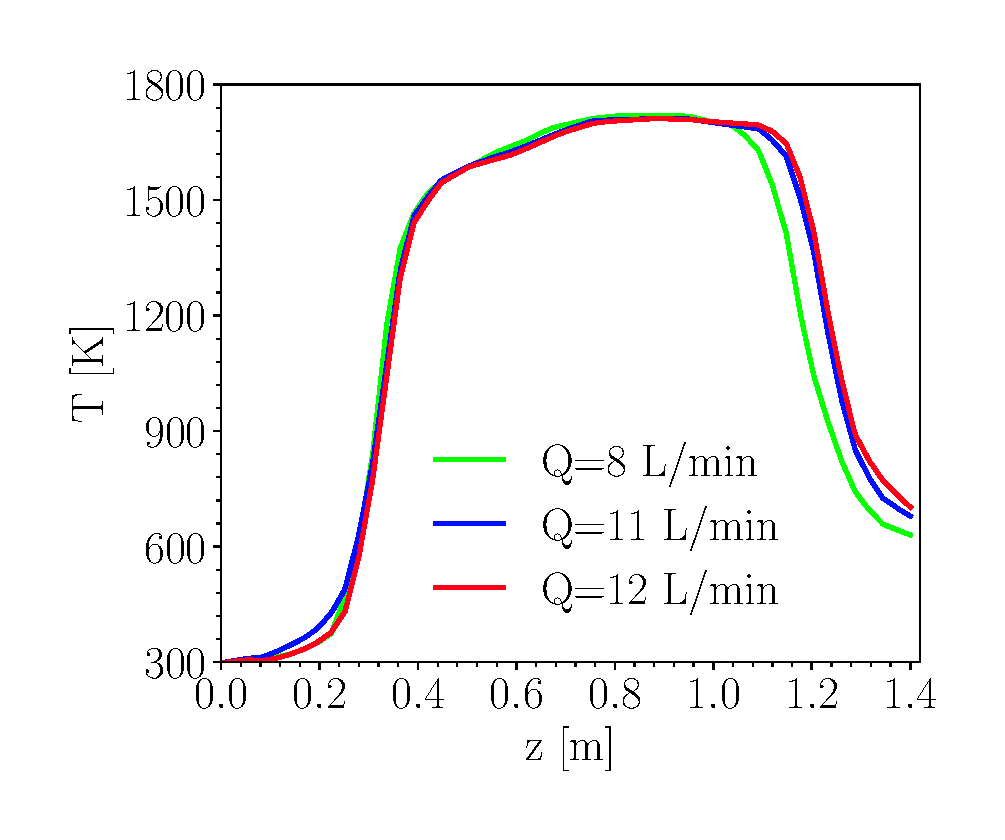
\includegraphics[width=0.45\textwidth]{Figures/Results/PFR/temperature_combined.pdf}
	\caption{The centerline temperature along the reactor for Q=8, 11, and 12 L/mi interpolated from the thermocouple measurements~\citep{mei2019quantitative}. The yellow area represent the region with temperature larger than 1200 K.}
	\label{fig:pfr_temp} 
\end{figure}

\begin{figure}[H]
	\centering
	\begin{tikzpicture}
		\draw (0, 0) node[inner sep=0] 	{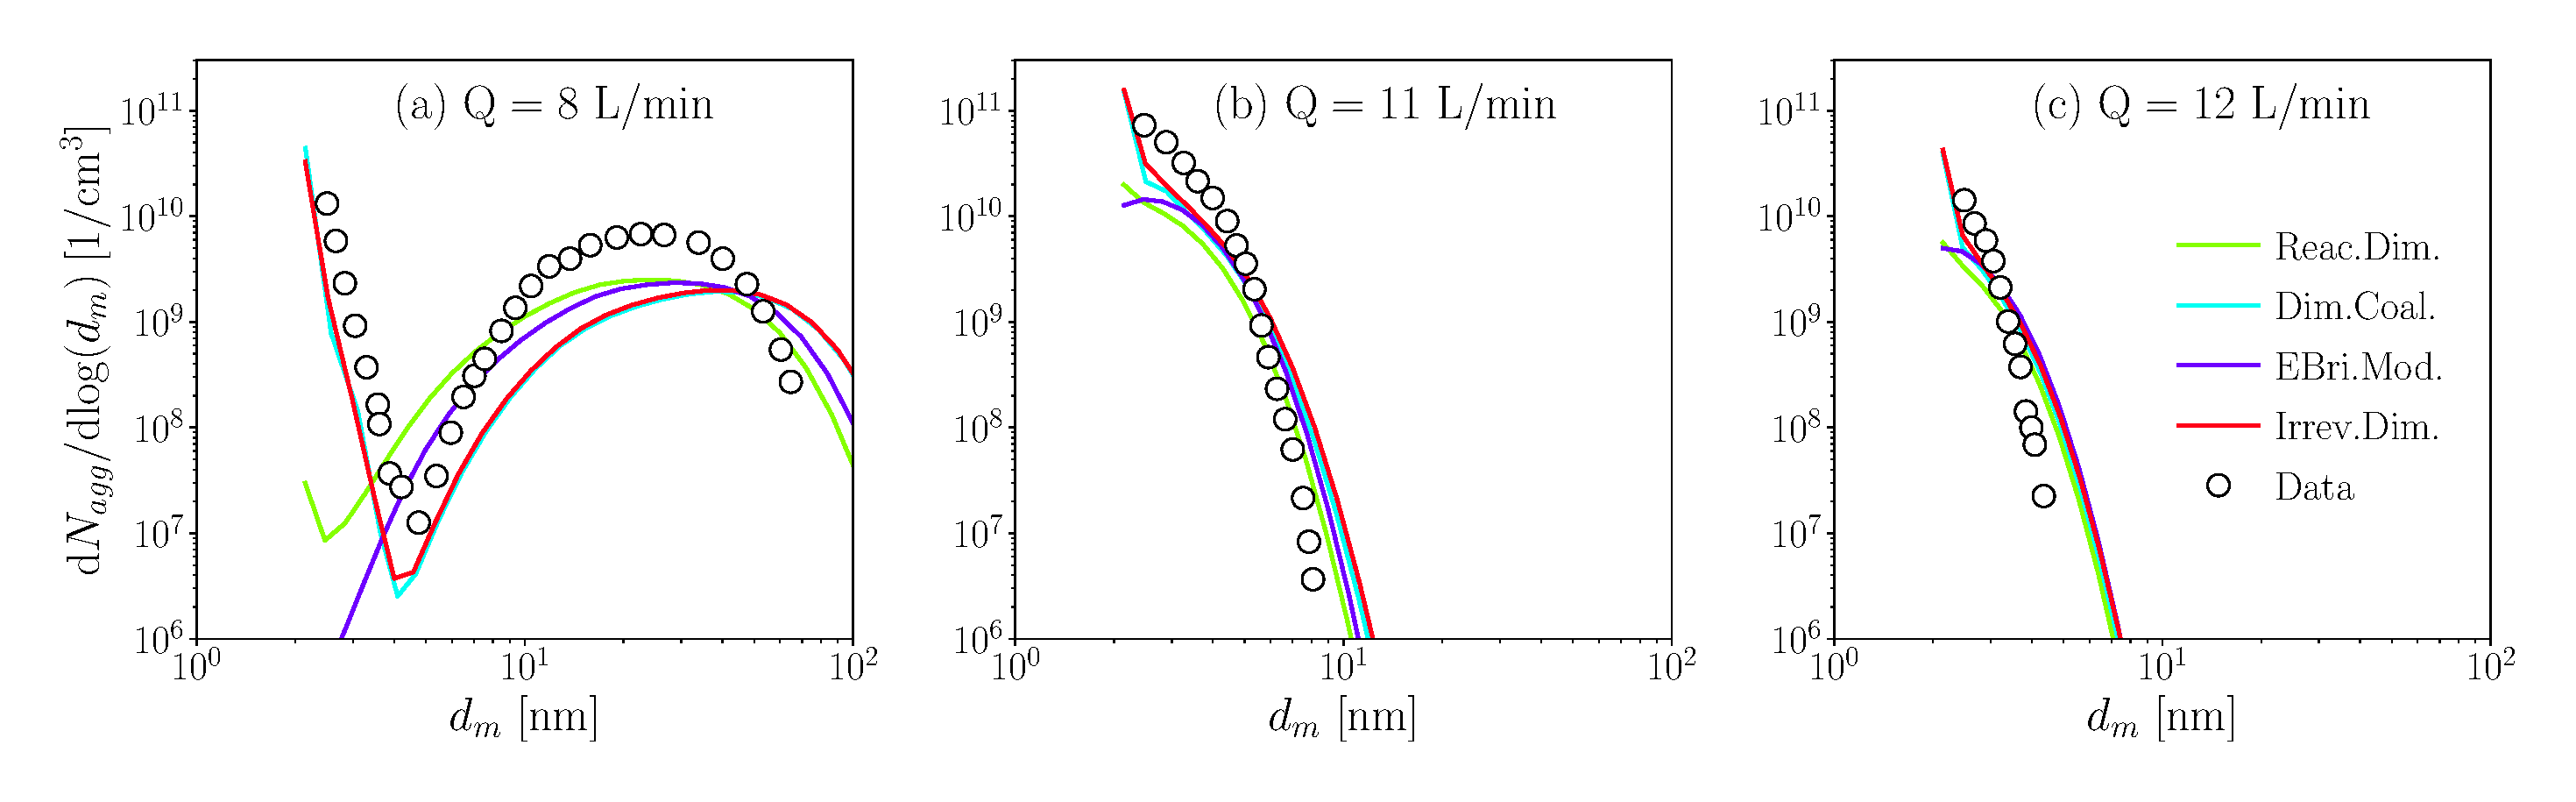
\includegraphics[width=1\textwidth]{Figures/Results/PFR/PSD_diffQ.pdf}};
		%\draw (-3.05, -1.1) node {\tiny{\cite{mei2019quantitative}}};
		%\draw (1.77, 0.59) node {\tiny{\cite{mei2019quantitative}}};
		\draw (6.63, -0.51) node {\scriptsize{\cite{mei2019quantitative}}};
	\end{tikzpicture}
	\caption{The particle size distribution at the end of PFR for Q=8.5 (a), 11 (b), and 12 L/min (c) obtained using KAUST mechanism and different inception models calibrated to match the predictions with measurement~\citep{mei2019quantitative}.}
	\label{fig:pfr_psd} 
\end{figure}

\begin{figure}[H]
	\centering
	\begin{tikzpicture}
		\draw (0, 0) node[inner sep=0] 	{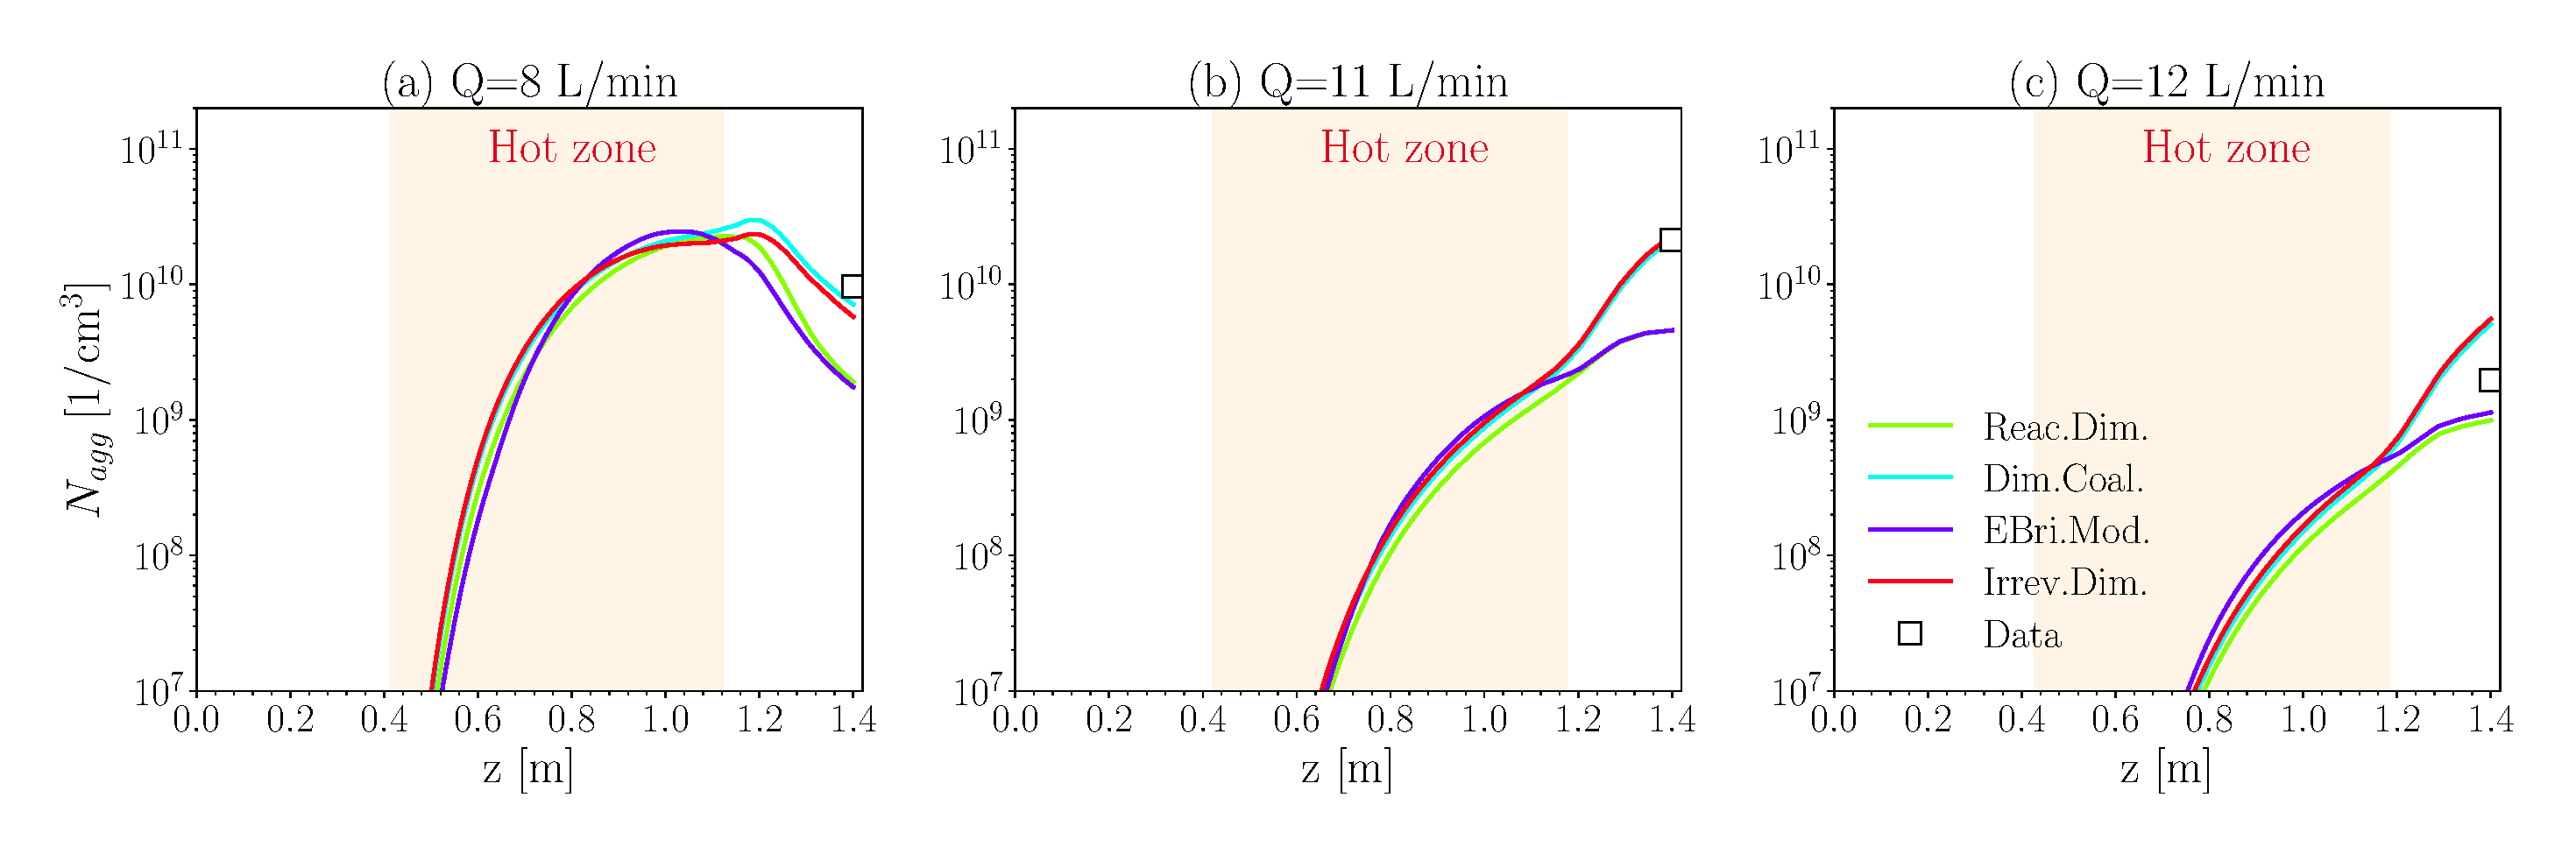
\includegraphics[width=1\textwidth]{Figures/Results/PFR/N_agg.pdf}};
		\draw (4.85, -1.1) node {\tiny{\cite{mei2019quantitative}}};
	\end{tikzpicture}
	\caption{The total number of agglomerates along the PFR for Q=8.5 (a), 11 (b), and 12 L/min (c) obtained using KAUST mechanism and different inception models compared with data~\citep{mei2019quantitative}.}
	\label{fig:pfr_Nagg} 
\end{figure}

\begin{figure}[H]
	\centering
	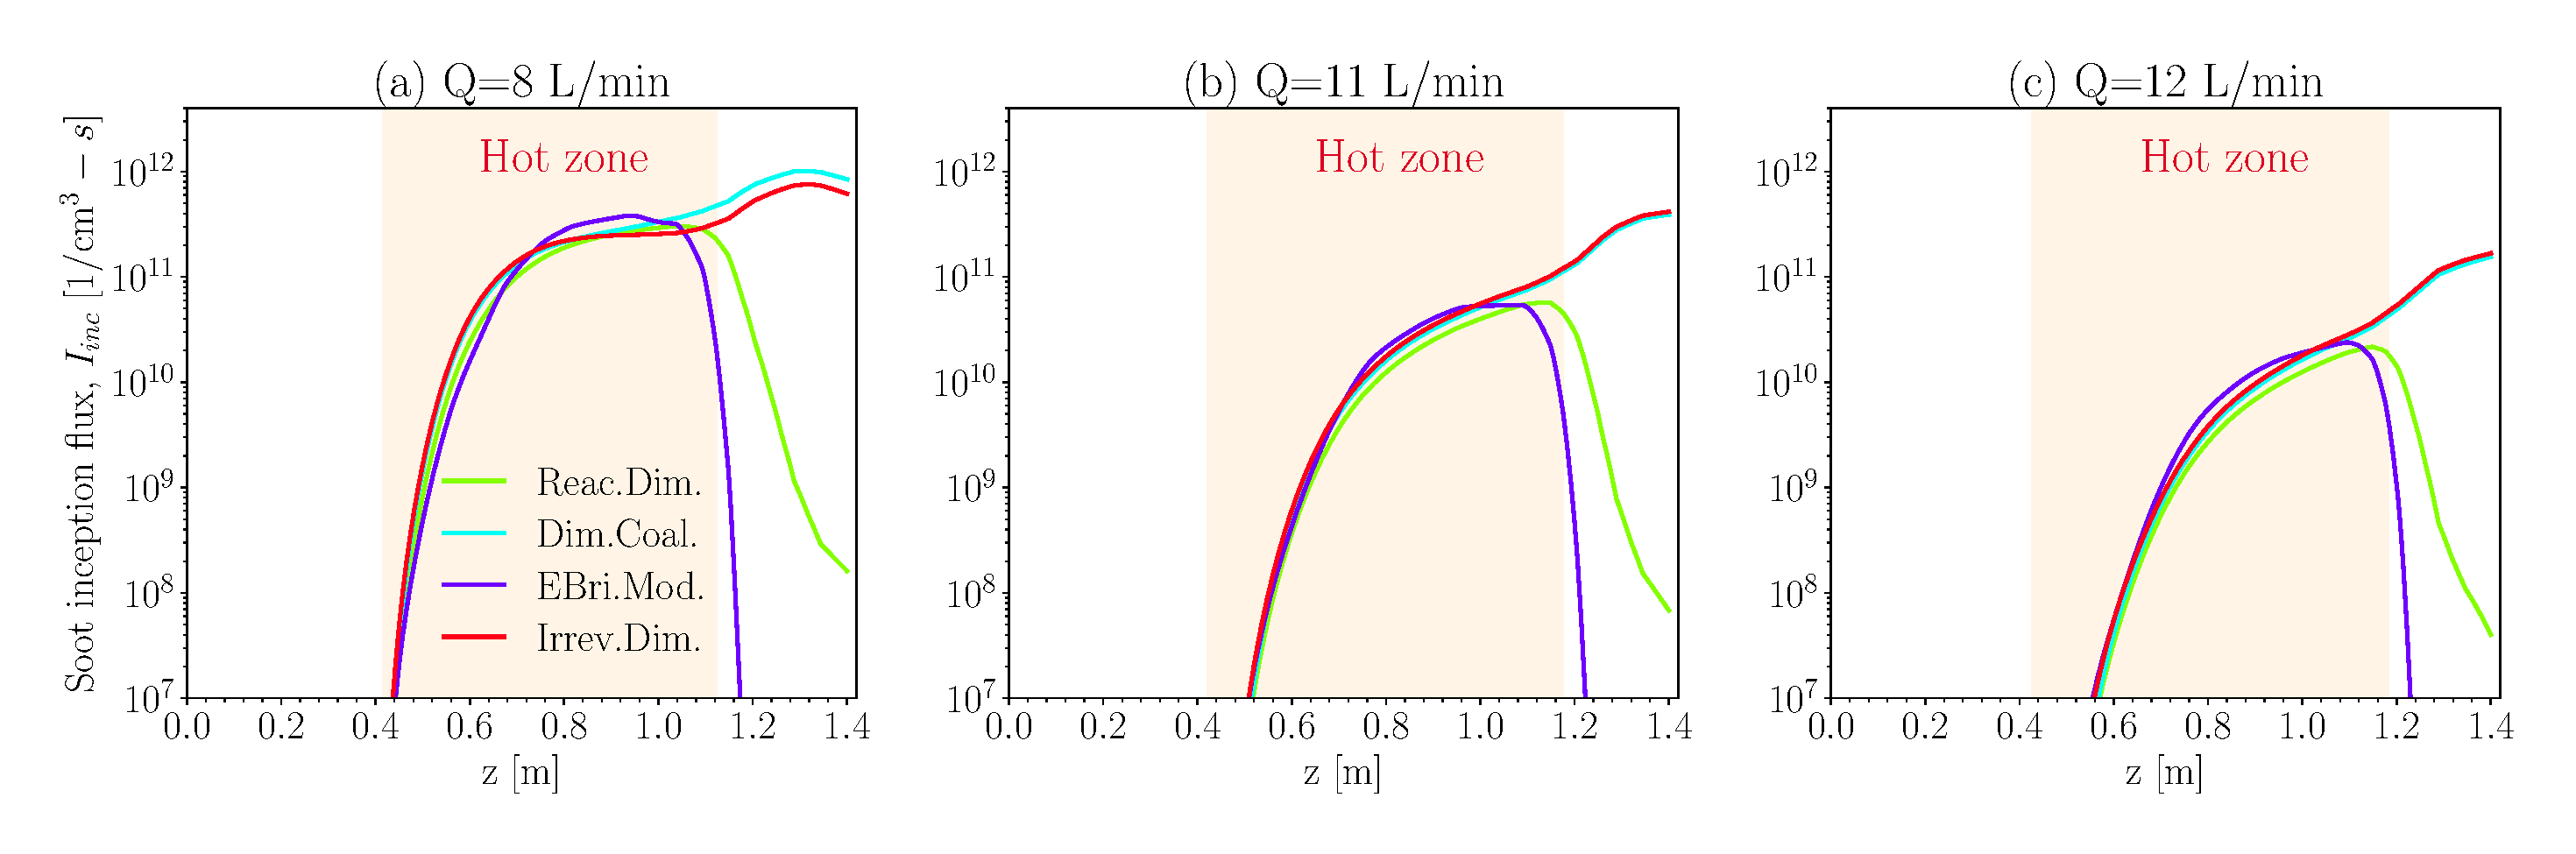
\includegraphics[width=1\textwidth]{Figures/Results/PFR/inception.pdf}
	\caption{The soot inception flux along the PFR for Q=8.5 (a), 11 (b), and 12 L/min (c) obtained using KAUST mechanism and different inception models.}
	\label{fig:pfr_Iinc} 
\end{figure}